\section{Software Design}

\paragraph{}
Most of the scope of this project was related to the software and firmware design and implementation.
This section details the design of the software, it's implementation, as well as issues encountered and how they were addressed or what needs to happen to address the issue in the future.

\subsection{High-Level Design and Implementation}

\paragraph{}
The software for this DAQ is designed and implemented to be run in a pseudo-parallel manner.
This means that several different tasks run sequentially, with each task running small chunks or sub-tasks during each cycle.
Each task is then designed as a state machine to segment itself into these smaller sub-tasks.
In order for each of these tasks to communicate with each other, there is one group of data that each task can reference.
Since this is a sequential action still, conflicts will not occur, and there does not need to be any extra protection for accessing the same data or variable at the same time.

\paragraph{}
The DAQ runs four main tasks that are continuously cycled through:
\begin{itemize}
	\item[(1)] Storage
	\item[(2)] Communication
	\item[(3)] Radio Communication
	\item[(4)] Sensors
	\item[(5)] Health Monitoring
\end{itemize}
The storage task is responsible for the actual logging of data.
The communication task is the task responsible for reading data off the CAN bus.
The radio communication task is responsible for medium-long range telemetry.
The sensors task is responsible for the reading of all on-board sensors.
The health monitoring task is responsible for updating any LED indicators for the health of the system.
Together, these five main tasks handle the running of all parts of the system.
As can be seen in \cref{fig:SoftwareTasks}, these tasks all run sequentially before looping back to the start.

\begin{figure}[H]
	\centering
	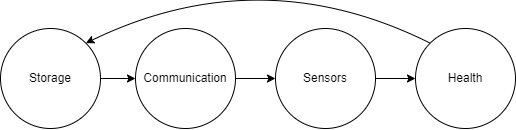
\includegraphics[width=0.75\linewidth]{SoftwareTasks.png}
	\caption{Software tasks loop diagram}
	\label{fig:SoftwareTasks}
\end{figure}

\paragraph{}
Object-oriented programming (OOP) is utilized significantly for this design.
Every task and sensor are a class that has individual constructors depending on the needs of the task.
Additionally, each task gets its own enum classes to define the various states for each state machine.
Two parent classes are utilized by everything.
For different tasks, there is an abstract task class that forces an implementation for a function that runs the task and requires the intercommunication data to be passed in.
For sensors, there is an abstract sensor class that forces an implementation for two functions: an initialization function and an update function.
Additionally, this class implements a read function that returns the current sensor value.

\paragraph{}
Since this project is based on the Arduino platform, several of the basic tasks for interacting with the hardware are handled by the platform.
This includes things such as setting the mode of a pin, reading and writing from data registers, configuring UART, SPI, and SDIO interfaces, and configuring the interrupt vector table.
Even with the configuration of these peripherals being handled by Arduino, they still need to be configured with the proper settings to be used.
Despite all falling under the Arduino umbrella, each platform is maintained independently of the others.
The people maintaining the Arduino platform for Teensy and the people maintaining the Arduino platform for STM do not communicate with each other, and as a result, there are some implementation differences that exist between different hardware platforms using Arduino.

\paragraph{}
Additionally, not every family of microcontroller from STM receives the same support or even the same supported functions from the Arduino framework.
One specific issue that arose was a versioning issue for STM32duino.
In version 18.0.0 and onwards, the memory sizes of the H7 family of STM microcontrollers were updated incorrectly, causing code to not run and the debugger to be unusable.
This issue was resolved by reverting the version of STM32duino back to 17.6.0.
The PlatformIO team has been notified of this issue and has responded that they are working on a fix.
Other issues that arose that were not issues on the Teensy platform were the signedness of pins on the STM32, multiple timers on the same timer channels, timer registers having different sizes, and the same interrupt being tied to multiple pins.
One of the largest benefits of this change was having access to the debugger.
Without access to a debugger, many of these issues would not have been solved or would have taken weeks or longer to debug.

\paragraph{}
The last main component that impacts each part of this system is a shared data segment.
This shared data segment is what allows all the tasks to communicate with each other.
Specifically, this includes variables for storing all the data that needs to be logged, flags for indicating when data has been updated, and fault flags to indicate when a task is encountering problems.
Since this code runs sequentially, there are no issues of different tasks attempting to read from or write to the same chunk of the shared data section at the same time.
As a result, there are no added protections for this scenario.

\begin{figure}[H]
	\centering
	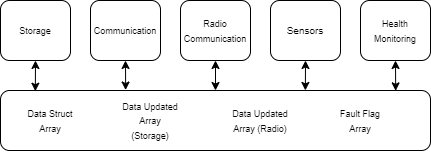
\includegraphics[width=0.75\linewidth]{SharedData.png}
	\caption{Shared Data Section Diagram}
	\label{fig:SharedData}
\end{figure}

\subsection{Storage Task}

\paragraph{}
The first and foremost task that the DAQ runs is the storage task.
This task is responsible for managing the SD interface as well as managing the filesystem.
This includes things like initializing the communication interface with the SD card, setting up the filesystem, and writing data to the SD card.

\paragraph{}
As with all tasks, this was implemented via a state machine.
A diagram for this state machine can be seen in \cref{fig:StorageDiagram}.
This machine consists of seven states, with each state handling a single part of the task.
These states are:
\begin{itemize}
	\item Initialize
	\item Wait to Open
	\item Open
	\item Wait to Write
	\item Write
	\item Close
	\item Error
\end{itemize}
In this state machine, there are two types of states.
These are action states and waiting states.
The action states are all capable of entering the error state if their action fails unexpectedly.
The waiting states are incapable of entering the error state, since their sole purpose is to wait for certain conditions needed for their corresponding action state.

\begin{figure}[H]
	\centering
	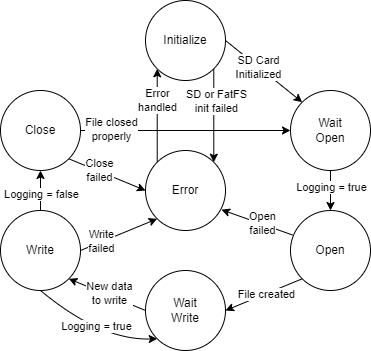
\includegraphics[width=0.75\linewidth]{SDStateMachine.png}
	\caption{Storage State Diagram}
	\label{fig:StorageDiagram}
\end{figure}

\paragraph{}
The Initialize state is responsible for creating the SD instance.
This includes configuring the SDIO communication interface that physically connects the SD card to the microcontroller as well as mounting the FatFS file system that is used by the SD card.
The creation of the SD and File objects relies on STM32SD library \cite{STM32SDGithub}.
This library provides the functions for initializing the SD interface and for mounting the file system.
One major issue is present in this library that needed to be fixed.
The library expects the FatFS implementation to have a function f\_unmount, which can be used to unmount the filesystem.
This function is not present in the FatFS implementation provided by STM32duino.
To resolve this issue, the function call can be replaced with a f\_mount function call with the appropriate arguments, or a wrapper function f\_unmount can be created that calls f\_mount with the appropriate arguments.
The former was used in this project.
If the returns of both the SD initialization and the FatFS initialization are success codes, the next state is Wait to Open.
If any other codes are returned, the next state is the Error state.

\paragraph{}
The wait to Open state is a waiting state that holds the storage task until the logging flag is high.
If the logging flag goes high, the next state is Open.
The task can be held in this state indefinitely if the logging flag stays low.
This can occur if the logging switch on the dashboard is disabled or removed.

\paragraph{}
The Open state is responsible for the creation of files.
Once the task enters this state, it searches for the next available file name and attempts to create the file.
The file is created and opened properly if the return of the open function, which is a wrapper around the FatFS f\_open function, returns a non-null value.
This state will attempt to open a file three times before deciding it is unable to.
If the file is opened properly, the next state is the Wait to Write state.
If the state is unable to open a file, the next state is the Error state.

\paragraph{}
The Wait to Write state is another waiting state that holds the storage task until new data is received.
Once a new piece of data is received from the CAN bus or from reading the onboard sensors, this state transitions to the Write state.
If there are no nodes on the CAN network or a CAN error and all the onboard sensors are disabled, the storage task can be held indefinitely in this state.
It is determined that a piece of data is new by checking a boolean value for each data segment.
These booleans are set to true in the communication task or the sensors task.

\paragraph{}
The Write state is responsible for writing the most recent data to the SD card.
Once the task enters this state, it iterates through all possible pieces of data to see if they have been updated.
If a piece of data has been updated, a data packet is created with the data ID, the data, and then a checksum to improve resiliency.
This packet is then written to the SD write buffer.
Once all updated messages are written to the SD write buffer, the buffer is then flushed to the SD card.
This is done on each iteration as opposed to waiting for the buffer to fill up to reduce the blocking when writing to the disk, to reduce the potential risk of missing data updates.
This is outlined in \cref{fig:SDWrite}.
If the writes and flush are completed successfully and logging is true, the next state is Wait to Write.
If the writes and flush are completed successfully and logging is false, the next state is Close.
If the writes or flush fail, the next state is Error.
Once the writes are complete, the booleans that are true for a data segment are reset to false.

\begin{figure}[H]
	\centering
	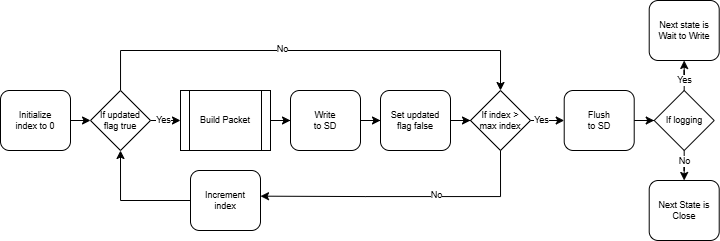
\includegraphics[width=\linewidth]{SDWrite.png}
	\caption{SD Task Write State Block Diagram}
	\label{fig:SDWrite}
\end{figure}

\paragraph{}
The final normal state is the Close state.
This state is responsible for safely closing the current open file.
If the file fails to close properly, the next state is the Error state.
To do this, any data remaining in the buffer is flushed to the SD card, and the File object is closed.
If the file closes properly, the next state is the Wait to Open state.
If the final flush fails or the file fails to close, the next state is set to the Error state.

\subsection{Communication Task}

\paragraph{}
The next task is the communication task.
This task is responsible for configuring and managing communication on the CAN bus.
To do this, the ACANFD\_STM32 library \cite{ACANFDGithub} was modified to support the operations needed to configure the CAN controller into CANFD mode and to read and write from the bus.
One requirement of this library is that the CAN IRQ handler functions need to be defined by the user.
These functions are defined in the main file and must be named properly to use the proper CAN controller, such as adding a 1 or 2 to distinguish between CAN1 and CAN2 hardware.

\paragraph{}
The state machine for the communication task contains four states.
These states are:
\begin{itemize}
	\item Initialize
	\item Wait for Message
	\item Process Message
	\item Error
\end{itemize}
As can be seen in \cref{fig:CommsDiagram}, the two main states which will be looped between are the Wait for Message and Process Message states that handle reading and processing messages.

\begin{figure}[H]
	\centering
	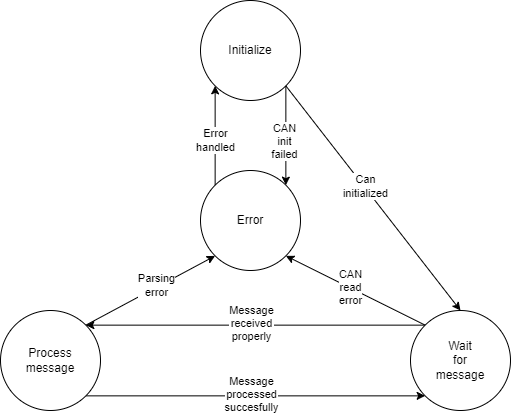
\includegraphics[width=0.75\linewidth]{CommsStateMachine.png}
	\caption{Communication State Diagram}
	\label{fig:CommsDiagram}
\end{figure}

\paragraph{}
The Initialize state is responsible for configuring the settings and initializing the CAN controller into CAN FD mode.
To configure the hardware into CAN FD mode, the pins that connect from the internal CAN controller to the external CAN transceiver need to be set to their alternate functions, and the bits in the configuration register need to be set to Normal FD mode.
Additionally, the desired arbitration clock rate and data clock rate need to be set as well, so that the bus is transmitting at the desired speed.
If there are no issues when configuring the CAN controller, the next state is set to Wait for Message.
If there are any issues, the next state is set to Error.

\paragraph{}
The Wait for Message state is the state that is directly responsible for reading data off the CAN bus.
If the CAN bus has a message available to be read, it reads the contents into a message variable.
If no messages are ever received, it is possible to become stuck in this state indefinitely.
If a message is received, the next state is set to Process Message.
If there are errors reading the message, the next state is set to Error.
Only one message will be read in this state, so if there are multiple messages ready to be read, the system will need to enter this state multiple times.

\paragraph{}
The Process Message state is responsible for taking the data from a received CAN message and moving it into the section of data shared by all tasks.
Additionally, to indicate to the storage task that a piece of data is new, an array of booleans that is equal in size to the number of data blocks exists.
When a message is received, the boolean that corresponds to the same integer value as the index of the received data block is updated to true.
This boolean will be reset to false in the storage task.
As is detailed in \cref{fig:CANProcess}, this state first checks if the CAN ID of a message is valid, something expected or able to be handled.
It then copies the contents of the CAN message into the corresponding data segment in the shared data.
Since it is expected that the CAN messages will fully correspond to the data segment and that the data segment will be byte aligned with no gaps, a simple memcpy operation can be done to move the data from the received message into the shared data.
If this processing is completed without error, the next state is set back to Wait for Message.
If there are any issues with the CAN message or the copying of the data, the next state is set to Error.

\begin{figure}[H]
	\centering
	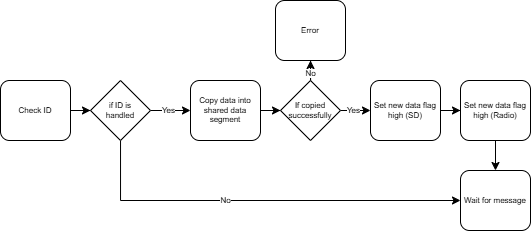
\includegraphics[width=0.75\linewidth]{CANProcess.png}
	\caption{CAN Message Processing Block Diagram}
	\label{fig:CANProcess}
\end{figure}

\paragraph{}
The final state of the communication task is the Error state.
This state is responsible for handling any errors that occur because of initialization, reading CAN messages, or processing the CAN messages.
The most common errors that can occur are the bus failing to initialize properly, and an invalid or unhandled CAN message IDs are received.
The most likely cause of the CAN hardware not initializing properly is improper wiring on the PCB or invalid configuration options or settings.
In either of these scenarios, recovery is not possible, and the task must be held in the Error state.
In the event of an invalid CAN ID received, the system can continue to operate successfully, and the task can be recovered by returning to the Wait for Message state.
In the shared data, a flag is set hig,h indicating a fault in the communication task.

\subsection{Radio Communication Task}

\paragraph{}
The radio communication task handles communication with the radio module and the transmission from the vehicle to the pit area.
The Xbee module handles the over-the-air transmission of data.
The Xbee module is configured separately, before being installed into the DAQ, accepting a UART communication line and relaying that data over the error.
The module is not configured to handle lost packets, invalid packets, or any issues related to the data transmission, as dropping packets is not a catastrophic failure.

\paragraph{}
The radio communication task has five states:
\begin{itemize}
	\item Initialize
	\item Wait
	\item Build
	\item Send
	\item Error
\end{itemize}
The state machine describing how to transition between these states can be seen in \cref{fig:RadioDiagram}.
Similarly to the storage task, there is a wait state whose only function is to hold the task until a certain condition is met.
This is the only state that cannot enter the Error state.

\begin{figure}[H]
	\centering
	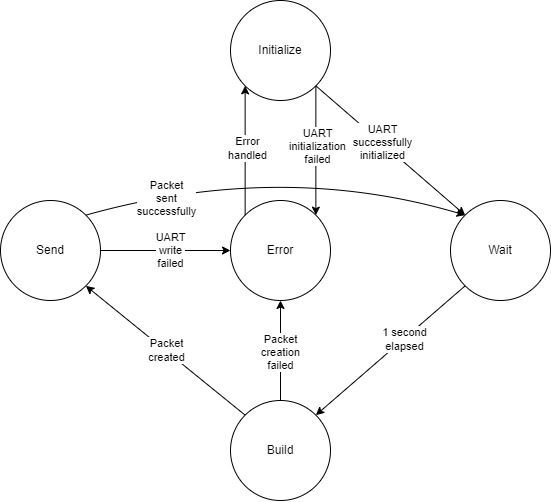
\includegraphics[width=0.75\linewidth]{RadioStateMachine.png}
	\caption{Radio Communication State Diagram}
	\label{fig:RadioDiagram}
\end{figure}

\paragraph{}
The Initialize state is responsible for configuring the UART communication interface with the Xbee radio.
The Arduino HardwareSerial library handles configuring the registers to their alternate functions, so long as the proper tx and rx pins are set.
The baud rate is configured to 57600 bits per second to comply with the Xbee's configuration.
If UART initializes successfully, the next state is the Wait state.
If the UART communication is not initialized successfully, the next state is the Error state.

\paragraph{}
The Wait state holds the radio communication task until it is time to send a packet over-the-air.
If a one second timer has triggered, the next state is the Build state.

\paragraph{}
The Build state is responsible for creating a single packet that will then be transmitted over-the-air.
Similarly to the storage task, this state checks which data segments have been updated and adds each segment that has been updated to the packet.
The data ID and the length of data are added before each data segment, and a checksum is computed and added to the end of the data segment.
Differently from the storage task, each updated data segment is added to a single packet.
If the packet is created successfully, the next state is the Send state.
If there are issues creating the packet, the next state is the Error state.

\paragraph{}
The Send state writes the created packet over UART to the Xbee module.
To reduce issues related to filling up the hardware buffer, the UART writes just a single byte at a time.
Additionally, there is a check to ensure that the hardware buffer is not full and can accept the byte.
The reason for this is that the write function that puts a byte or array of bytes onto the hardware buffer does not check if the buffer is full, and it will hold the program until the byte or bytes in the array are written to the buffer.
This makes it very likely to cause interruptions in the code, harming the running of the other tasks.
Once all bytes are written to the buffer, the next state is set back to the Wait state.
If there are any issues with writing a byte, the next state is the Error state.

\paragraph{}
The last state in the radio communication task is the Error state.
Similarly to the communication state, if there are any issues setting up the UART communication line, it is likely a result of faulty wiring or invalid parameters.
In this event, the error is typically not recoverable.
If the error occurs within the Build or Send state, the error can be recovered.


\subsection{Sensors Task}

\paragraph{}
The sensors task is responsible for reading the DAQ's onboard sensors.
These sensors include the onboard IMU and GPS, as well as a few analog sensor inputs.
The IMU and GPS both communicate over I2C, and the analog sensors utilize the internal ADC of the STM32.
These sensor readings are then added to the shared data section so that they can be written to the SD card.

\paragraph{}
This task has five states:
\begin{itemize}
	\item Initialize
	\item Wait
	\item Read
	\item Send
	\item Error
\end{itemize}
The state machine describing the transitions can be seen in \cref{fig:SensorsDiagram}.
Similarly to the radio tasks, there is a time-based waiting task and four additional tasks for functionality.
Different from the radio communication task is that there will be two states that cannot enter the error state, the Wait state and the Send state.

\begin{figure}[H]
	\centering
	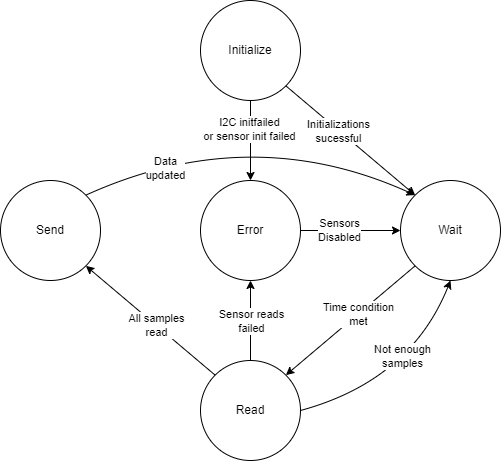
\includegraphics[width=0.75\linewidth]{SensorsStateDiagram.png}
	\caption{Sensors State Diagram}
	\label{fig:SensorsDiagram}
\end{figure}

\paragraph{}
The Initialize state is responsible for configuring the peripherals needed to communicate with sensors and for configuring any sensors when it is applicable.
Since both the IMU and GPS communicate over I2C, two I2C buses need to be configured.
Additionally, each of these sensors need to be configured, including items such as setting up the sampling rate, any on board filtering, or changing the sensor range.
For the basic analog sensors, the pins need to be configured to use their ADC alternate function.
The Arduino pinMode function takes care of this.
Additionally, the bit resolution also needs to be configured.
To comply with the requirements of this project, this must be at least 10 bits.
If everything is configured properly, the next state is the Wait state.
If there are any issues, the next state is the Error state.

\paragraph{}
The Wait state holds the task for a specified amount of time.
The purpose of this is to ensure that sensors are sampled at fixed intervals to support digital filters.
As a result, the amount of time the task is held in this state is determined by the desired sampling rate of the sensors which pre-processing filtering is done on.
Since the only thing this state does is wait for a time condition to be met, it is impossible to fault, and, as such, cannot enter the Error state.
Once the time condition is met, the next state is the Read state.
If no pre-processing of the data is done, the time held in this state is 0, and the next state is immediately set to be the Read state.

\paragraph{}
The Read state is responsible for reading the data from sensors.
To do this, the analog channels need to be sampled, and samples need to be requested from the sensors communicating over I2C.
Each sensor is only sampled if there were no issues with the configuration of the sensor.
If any pre-processing is desired, it will occur in this state directly after reading a sensor's sample.
At this point, there is no pre-processing, so there are no filter implementations directly on-board the DAQ.
If all sensors are sampled without issue and the number of samples taken is equal to the number of samples needed for a filter, the next state is set to the Send state.
If the sensors are all sampled without issue, but the number of samples taken is fewer than the number of samples needed for a filter, the next state is the Wait state.
If there were any issues sampling the sensors, the next state is set to be the Error state.
Issues can arise if there is no response to a request from an I2C sensor, or if an analog sensor returns a value outside of its expected range.
If there is no pre-processing of data, each time the sensors are sampled, the next state will become the Send state.

\paragraph{}
The Send state is a simple state that updates the data in the shared data section and sets the flag that this data is new to true for the storage task and radio communication task.
Since the code is sequential, there are no risks of conflicts arising from different tasks reading or writing at the same time.
As a result, it is not possible for this state to fault, and as a result cannot enter the Error state.
Once the shared data section is updated and the flags indicating that the data is new are set to be true, the next state is set to the Wait state.

\paragraph{}
The Error state handles any issues that arise from configuring the communication with sensors, the configuration of the sensors themselves, or sampling of the sensors.
If the communication interface fails to initialize properly, it is unlikely to be resolved.
A flag is set in the shared data section to indicate this.
However, if any of the communication interfaces initialize properly, the task is recoverable, and receiving some of the data is better than receiving none of the data.
The same is true of the sensors themselves.
If any of the sensors fail to initialize, a flag is set in the shared data section to indicate this, but the task can continue without this sensor.
Reading the sensors behaves similarly.
If a sensor fails to read properly, a flag is set in the shared data section, and the sensor is disabled in the Read state.
The state machine then recovers into the Wait state.

\subsection{Health Monitoring Task}

\paragraph{}
The health monitoring task detects and reports issues with the system.
This is done by toggling on-board LEDs to act as visual indicators in the event of issues.
These issues include things such as CAN failures, SD failures, and a heartbeat.

\paragraph{}
This task is the simplest state machine with just two states and no Error state.
These are the initialization state and the update state.
The diagram for this state machine can be seen in \cref{fig:HealthDiagram}.

\begin{figure}[H]
	\centering
	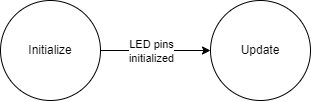
\includegraphics[width=0.75\linewidth]{HealthStateDiagram.png}
	\caption{Health Monitoring State Diagram}
	\label{fig:HealthDiagram}
\end{figure}

\paragraph{}
The initialization state is responsible for configuring the pins for LEDs.
Since all GPIO pins on an STM32 can be configured to be outputs, it is not possible to fail to initialize.
As a result, the next state is always set to be the Update state.

\paragraph{}
The update state checks the status of the other tasks and toggles LEDs as needed.
Additionally, the heartbeat is updated in this state.
Similarly to the initialization state, since this state is only performing digital writes, or updating the output data register, it is not able to cause a fault.
The heartbeat LED is toggled once every half second, for a total frequency of 1 Hz.
The indicator LEDs directly use booleans from the shared data section to write a value to the LED.
This means that the output of those LEDs is determined by the other tasks.
The health monitoring task remains in the update state for the entire time the system is running.